\documentclass[runningheads,a4paper]{llncs}
\usepackage[T1]{fontenc}
\usepackage{graphicx}
\usepackage{booktabs}
\usepackage{amsmath}
\usepackage{url}
\usepackage{textcomp}
\usepackage[hidelinks]{hyperref}
\raggedbottom
\begin{document}
\title{Sun / LA: Visualizing Sun Exposure and Underserved Bus-Boarding Reachability in Los Angeles}
\titlerunning{Sun / LA: Sun Exposure and Bus-Boarding Reachability}
\author{Tianyi Wang \and Yi-Fan Tsai \and Shuang Wu \and Yang Xu}
\authorrunning{T. Wang et al.}
\institute{University of Southern California, Los Angeles, CA, USA\\
\email{twang121@usc.edu}, \email{yifantsa@usc.edu}, \email{swu84271@usc.edu}, \email{yxu95543@usc.edu}}
\maketitle
\begin{abstract}
Sun / LA is a geovisualization dashboard that shows transit planners, shade advocates, and Los Angeles riders why a nearby bus stop can still be hard to board or exposed to direct sun, for 1,120 census-tract origins. It addresses two visualization challenges. First, one sun-exposure fill per tract cannot show whether sun falls on the walk or the wait, or separate missing data from shade; we link fixed-bin tract fills to orange/teal/gray route segments and a walk-and-wait breakdown. Second, street-level routes must stay legible over a fine-unit choropleth while walking time is kept apart from boarding difficulty, walk plus scheduled wait above 30 minutes; our reachability map shares one eight-class walking-time scale between fills and routes, adds dark casings, and draws default routes only for underserved tracts. At 08:00, 52 of 1,120 origins (4.6\%) are difficult to board.
\keywords{Transit accessibility \and Choropleth \and Route maps \and Sun exposure}
\end{abstract}

\section{Introduction}
A bus-stop pin cannot show whether a rider can walk there, board soon, or stay out of the sun. Planners need neighborhoods where walking plus waiting exceeds 30 minutes, and shade advocates need to know whether sun falls on the walk or at the stop to choose between trees and shelters. Metro reported shelters at 24\% of its stops in 2022~\cite{metro2022}, and shade in Los Angeles is uneven~\cite{reginald2024}.

\emph{Reachability visualization challenge.} Walking and boarding times exist in no dataset; we compute them by routing each origin and matching arrivals to timetables. It is hard to show: about 113,000 walks converge on shared streets above 1,120 tract polygons, walking time and walk-plus-wait are different measures, a route colored on the fills' scale vanishes on an area of its own class, and difficult tracts, 4--7\% of the city by day, are easily lost.

\emph{Primary visualization challenge: sun exposure.} Sun before boarding is also computed, from lidar heights and solar position at each six-second walking step and waiting minute. One fill per tract cannot say whether the walk or the wait is sunny, and missing data must not read as shade.

\emph{Contributions.} For each challenge we contribute a linked display and join both in one dashboard. Sections~\ref{sec:related}--\ref{sec:conclusion} cover related work, data, design, results, and limitations.

\section{Related Work}\label{sec:related}
\emph{Travel-time maps with routes.} Zeng et al.~\cite{zeng2014} derive transit journey times, including waits and transfers, from smart-card trips, and avoid geographic flow clutter by pairing an isochrone map with an isotime flow map that straightens routes along a time axis. Andrienko et al.~\cite{andrienko2020} summarize how well public transport connects places. These designs start from one source or aggregate routes; we start from every tract and keep real street paths on the fills' scale.

\emph{Sun and shade.} Shadow accrual maps~\cite{miranda2019} make city-scale shadow accumulation over long periods fast enough to explore, and the Urban Toolkit~\cite{moreira2024} composes shadow and other urban layers through a grammar. Both summarize shade over areas and periods; we sample one trip, a moving walk and a fixed wait at the chosen departure, and keep unresolved intervals gray.

\emph{Walking access and heat.} Real walks to stops differ from the 400\,m buffer~\cite{elgeneidy2014}, signals delay pedestrians~\cite{marisamynathan2018}, and waits drive riders' heat vulnerability~\cite{fraser2017}; Sun / LA shows these factors together.

\section{Data}\label{sec:data}
Table~\ref{tab:data} lists the inputs. The unit is the census tract (1,120), the smallest with reliable American Community Survey estimates, labeled with its \emph{Mapping L.A.} neighborhood name because readers recognize ``Tujunga,'' not ``Tract 1011.22.''

\begin{table}[!htbp]
\caption{Core inputs and their roles.}\label{tab:data}
\centering
\footnotesize
\begin{tabular}{@{}p{.3\linewidth}p{.65\linewidth}@{}}
\toprule
Source & Data and visualization role \\
\midrule
\href{https://download.geofabrik.de/north-america/us/california/socal.html}{OpenStreetMap}~\cite{osm} & Directed pedestrian network for walking paths and times \\
\href{https://gitlab.com/LACMTA/gtfs_bus}{Metro GTFS}~\cite{metrogtfs} & 10,968 stops; departures frozen to Oct.\ 27, 2026 \\
\href{https://maps.lacity.org/lahub/rest/services/LADOT/MapServer/30}{LADOT signals}~\cite{ladotsignals} & Mapped signal locations for assumed crossing delays \\
\href{https://www.census.gov/programs-surveys/acs/data.html}{ACS 2020--2024}~\cite{census2024} & Tract demographics for the Sun Exposure scatter plot \\
\href{https://wifire-data.sdsc.edu/dataset/nasa-werk-dem-ca-losangeles-1-b23}{NASA WERK lidar}~\cite{werk} & Terrain and surface heights (4\,m cells) for shade \\
\href{https://services1.arcgis.com/tp9wqSVX1AitKgjd/arcgis/rest/services/VMT_2022_by_LA_Times_Neighborhood_WFL1/FeatureServer/0}{Mapping L.A.}~\cite{mappingla} & LA Times neighborhood names for tract labels \\
\bottomrule
\end{tabular}
\end{table}

\section{Design and Implementation}\label{sec:design}
\emph{Computing reachability and sun exposure.} Walking time is the fastest Dijkstra path at 4.8\,km/h, plus 0 or an assumed 30\,s per mapped signal crossing. For each of 48 half-hour departures, time to board is the minimum, over stops within a 30-minute walk, of the walk plus the wait for the first scheduled departure. An origin is \emph{difficult to board} if this exceeds 30 minutes or its shortest walk alone does. Modeled sun exposure sums the sunlit walking and waiting intervals whose shade is known.

\emph{Reachability map design.} Riders reach a stop on foot, so we route on walkable OpenStreetMap streets and footways, excluding freeways and links closed to pedestrians. Each tract starts from one interior point (moved to a nearby street in 57 tracts), a reproducible origin. Walks to a bus are usually short~\cite{elgeneidy2014}, so 30 minutes, six times the median walk, is a conservative threshold. Fills encode walking time in eight classes, with breaks at 5, 10, 15, 20, 30, 45, and 60 minutes. The breaks follow the skewed data: 84\% of tracts walk under 10 minutes, one break sits at the threshold, and the classes beyond it hold the 29 tracts whose walk alone is too long. ColorBrewer YlGnBu colors~\cite{harrower2003} darken monotonically, so the order should survive grayscale and color-vision deficiency. A red ``!'' marks walk plus wait above 30 minutes.

Each route is colored by its own walking time on the same scale; a dark casing, plus a red edge for difficult tracts, keeps it visible on a fill of its own class (Fig.~\ref{fig:reach}b). Riders start from home, so by default only difficult tracts show routes, to their three closest stops; a click shows a tract's stops within 60 minutes or a stop's catchment, and toggles hide each layer. We rejected straight-line buffers, which ignore street barriers, and drawing all routes; an earlier blue-fill, red-route version read as two measures, and a purple edge sat 43\textdegree{} in hue from the 45--60 class, so we chose red, which a unit test keeps over 60\textdegree{} from every class.

\emph{Sun exposure design.} Fills use five fixed bins (0--5 to 20+ minutes). At summer 08:00 about 69\% of tracts fall in 0--5 and at noon 6\% exceed 20, so five-minute steps separate the common values, the open bin holds the long-wait tail, and fixed breaks keep seasons comparable. The yellow-to-red palette also darkens monotonically. The selected walk is orange (sun) or teal (shade) on a white halo that separates it from the fills; gray marks unknown, and routes appear only for the selection (Fig.~\ref{fig:sun}).

\emph{Layout and implementation.} Both views are map-first with a side panel giving one headline number, and two tabs keep walking and sun minutes off one color scale. In one React application (Fig.~\ref{fig:dash}), a parent component holds the selected neighborhood, tab, and search and passes them to both maps and a D3 scatter plot, whose dots select neighborhoods on the map. deck.gl draws the layers over a MapLibre basemap; Bootstrap styles menus and buttons. Offline Python scripts precompute routes and shade as JSON; routes (55.7\,MB in all) are split into one file per tract, about 9\,KB each, loaded on click. An AI coding assistant helped write and debug the React/TypeScript code and automated tests.

\section{Usage Scenarios and Results}\label{sec:results}
\subsection{Primary Challenge: Walking Versus Waiting Exposure}
In summer at 08:00, Hollywood (Tract 1902.01) has a fill in the lightest class, about 1.5 minutes, because the overview uses the stop with the earliest boarding. Selecting it shows the trip to its \emph{nearest} stop, Yucca/Cahuenga: a 1.3-minute walk, then a 52.7-minute wait in sun (Fig.~\ref{fig:sun}). This contrast is our evidence that a fill-only map hides wait exposure, and it points to a shelter, not trees.

\begin{figure}[!t]
\centering
\begin{minipage}[t]{.43\linewidth}\centering
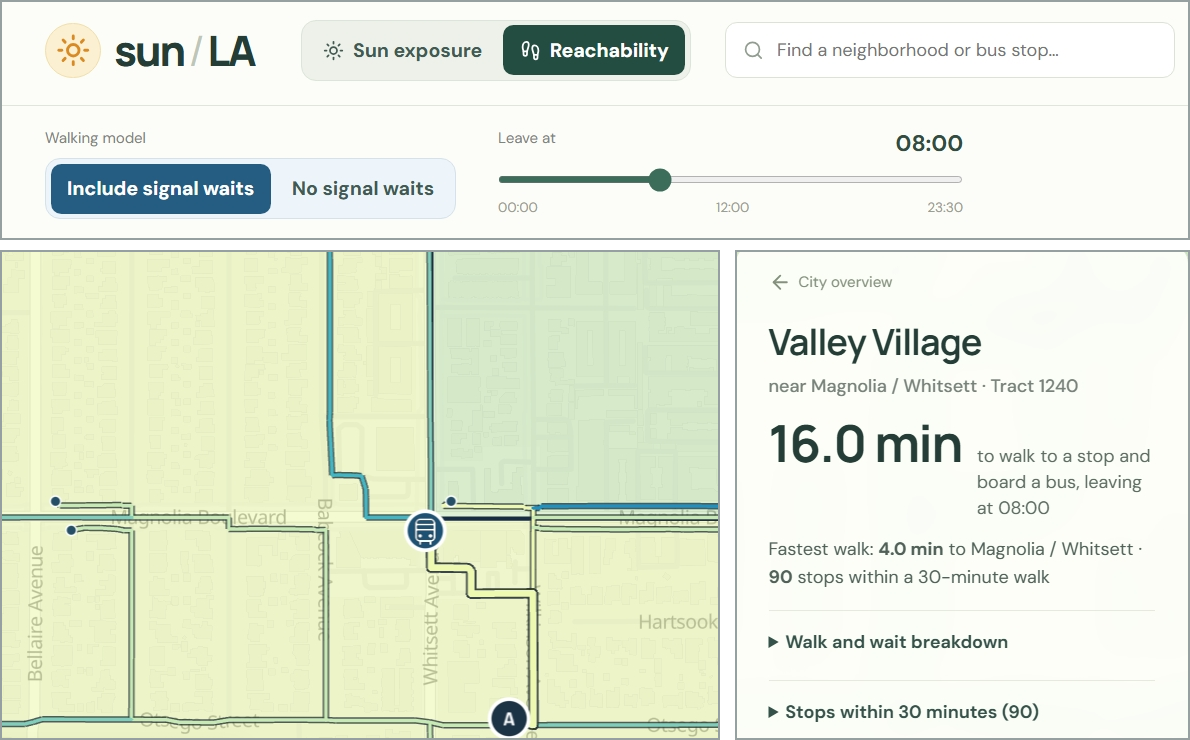
\includegraphics[width=\linewidth]{figures/fig1.png}
\caption{The dashboard: tabs, shared search, view controls, map, legend, and side panel.}
\label{fig:dash}
\end{minipage}\hspace{.04\linewidth}
\begin{minipage}[t]{.52\linewidth}\centering
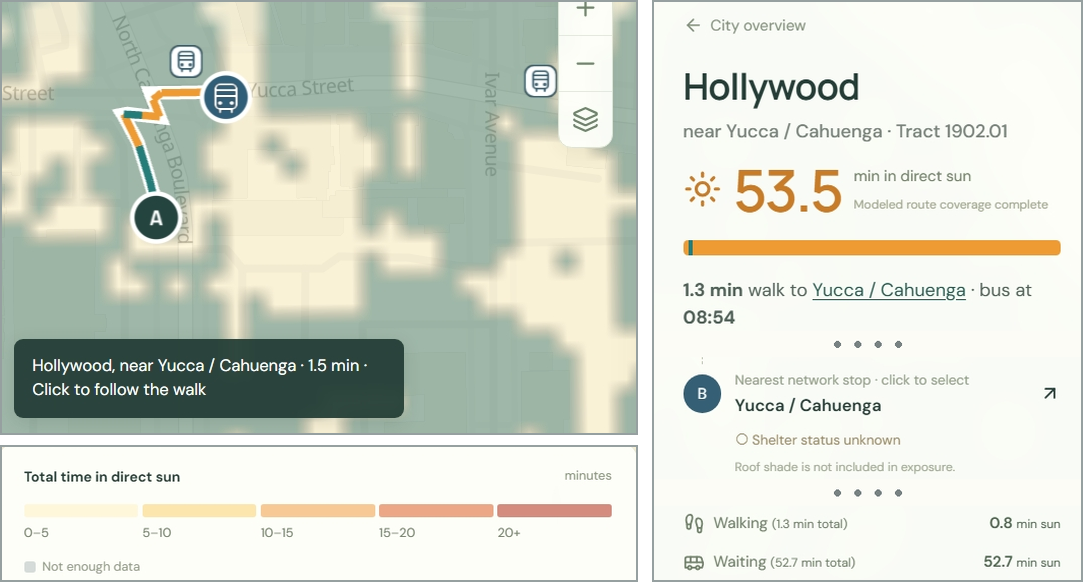
\includegraphics[width=\linewidth]{figures/fig2.png}
\caption{Hollywood, summer 08:00. Fills: sun minutes, yellow to red; gray = no data. Route: orange = sun, teal = shade, gray = unknown.}
\label{fig:sun}
\end{minipage}
\end{figure}

\subsection{Reachability Challenge: Walking Versus Boarding}
At 08:00 with signal delays, 52 of 1,120 origins (4.6\%) are difficult, 29 on the walk alone and 23 because of the wait, mostly in the hills, the north-west Valley, and near the harbor (Fig.~\ref{fig:reach}a). Tujunga (Tract 1011.22) needs 39.0 minutes; its 29:54 walk has the color of its own tract, and the casing keeps it readable (Fig.~\ref{fig:reach}b). The count stays at 44--78 by day but reaches 375 at 03:00, 346 of them from waiting. The signal delay makes Palms (Tract 2699.03) miss a 03:03 bus, moving boarding from 3.0 to 47.0 minutes (Fig.~\ref{fig:reach}c). A 400\,m buffer would call many of them served: 247 of the 346 are within a 10-minute walk.

\begin{figure}[!t]
\centering
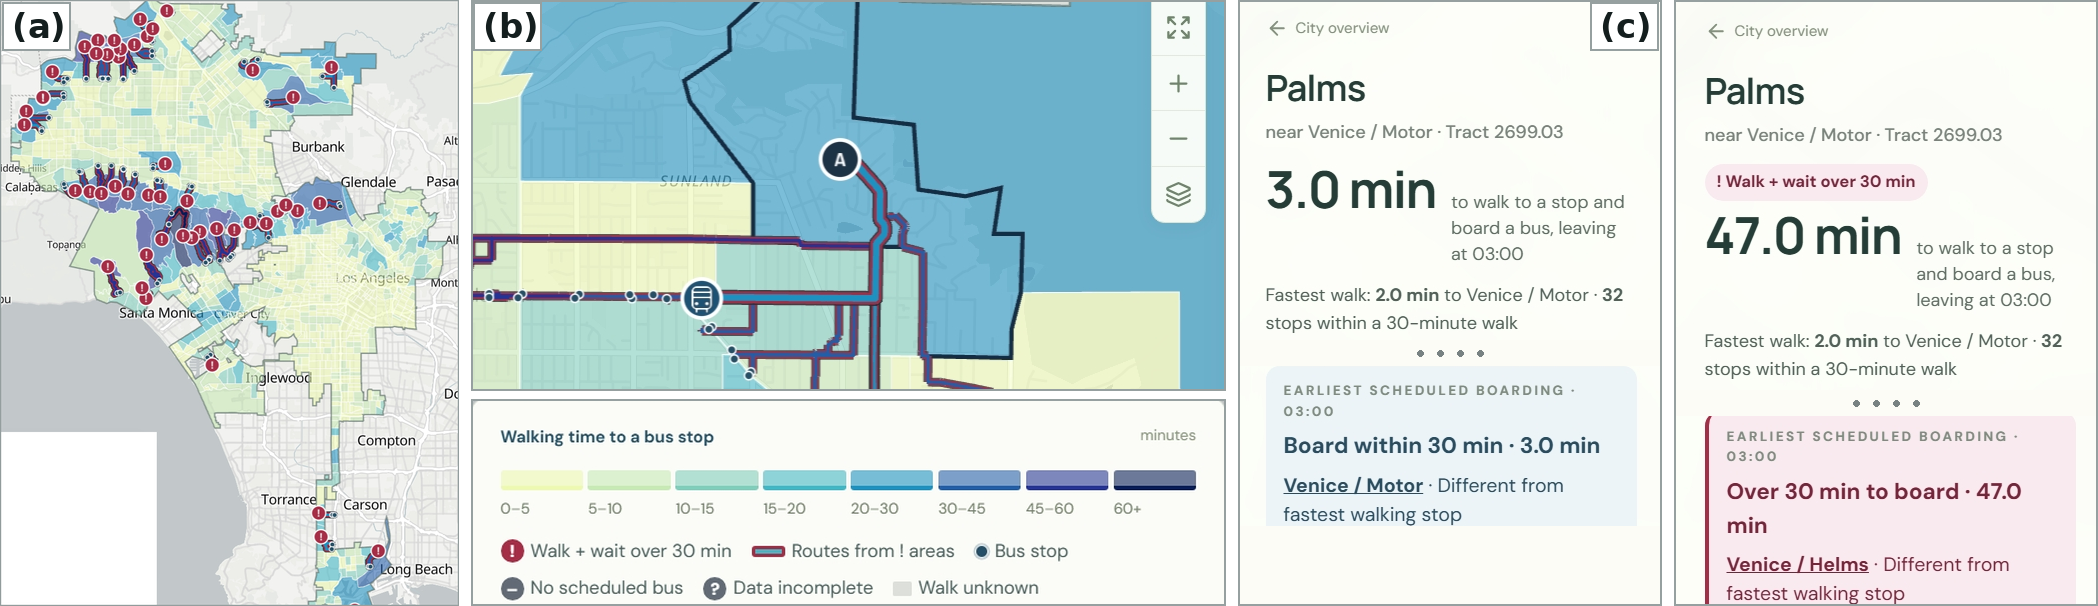
\includegraphics[width=\linewidth]{figures/fig3.png}
\caption{Reachability: fills and routes share one walking-time scale, light yellow (0--5 min) to dark blue (60+); red ``!'' = walk plus wait over 30 min. (a) 08:00. (b) Tujunga. (c) Palms at 03:00, without and with signal delays.}
\label{fig:reach}
\end{figure}

\section{Conclusion}\label{sec:conclusion}
Sun / LA separates proximity from access before boarding. Four limits shape what the maps show: one origin per tract can misstate large hillside tracts; the flat 30-second delay on mapped signals makes flags near 30 minutes sensitive; one weekday Metro schedule ignores other operators; and clear skies and unmodeled shelter roofs make sun minutes an upper bound. Outputs passed automated validators and an independent Dijkstra check. A four-task study (4--6 outside participants, fill-only versus linked view), color-vision checks, and field checks of the 1,617-point shelter list remain future work.

\bibliographystyle{splncs04}
\bibliography{mybibliography_5page}
\end{document}
